%-----------------------------------------------------------------------------
% Template for AIMS Rwanda Structured Masters Research Project
%
% The fonts, linespacing, numbering, page styles, order
% of  Title/Abstract/TOC/Body/{Appendices}/Acknowledgements/References 
% are prescribed as the AIMS house style.
%
% Do not change them or add to it without getting approval first.
% Essays are not accepted if they do not follow house style.
% This is in preparation for your Masters/PhD where the university
% will be much more strict on the house style.
%
\documentclass{aimsessay}
\usepackage[utf8]{inputenc}
\usepackage[round]{natbib}
%
%-----------------------------------------------------------------------------
% To use external packages for specific needs, 
% get approval before adding them here (they
% should not override general AIMS house style and layout).
%
% Examples:
%
% For Arabic
%\usepackage{arabtex}
%\usepackage{utf8}
%\setcode{utf8}
% For tables:
\usepackage{booktabs} % \toprule, \midrule, \bottomrule
\usepackage{array}    % \newcolumntype
% 
% For figures:
\usepackage[below]{placeins} % use \FloatBarrier in the body
% \usepackage{float}  %"H" placement spec, for **really here** (i.e. not float)
\usepackage{caption} %many figures in one figure (note subfigure and subfig are deprecated)
\usepackage{subcaption} %many figures in one figure (note subfigure and subfig are deprecated)
%
% For code and algorithms
\usepackage{moreverb}   % \verbatimtabinput
% For links and hyper references
\usepackage{hyperref}
\urlstyle{same}
% \usepackage{listings} % more flexible and complicated 
                        % than moreverb and algorithm
% 
% Others
% \usepackage[all]{xy} 
 \usepackage{sagetex}
% \usepackage{siunitx} % to typeset numbers, units, align decimals in tables.
% \usepackage{dcolumn} % less flexible but maybe faster than siunitx above.
% \usepackage{mathtools} % More maths, e.g. \mathclap.
\usepackage{epstopdf}
\usepackage{psfrag}
\usepackage{graphics}% Others may be landscape, longtable, algorithm, algorithmic, etc.
\usepackage{lineno} % This package together with lineno.sty numbers every line. Makes it easy for edditing.

% Numbers lines
\linenumbers
% 
%Saar-Tsechansky and Provost (2007b ----------------------------------------------------------------------------
% An AIMS Essay can use the sectioning commands "\chapter", "\section",
% "\subsection". No "\subsubsection", "\paragraph", etc. They are disabled.
% 
% For Theorems and such, use the environments defined here:
% \begin{thm}...\end{thm} (or "lem", "defn", etc)
% 
% We put the number to the left of the Theorem heading.
\swapnumbers 
% 
% Theorems are in italics.
\theoremstyle{plain}
\newtheorem{thm}[subsection]{Theorem}
%
% Rest is not in italics.
\theoremstyle{definition} 
\newtheorem{lem}[subsection]{Lemma}
\newtheorem{cor}[subsection]{Corollary}
\newtheorem{conj}[subsection]{Conjecture}
\newtheorem{pro}[subsection]{Proposition}
\newtheorem{exa}[subsection]{Example}
\newtheorem{defn}[subsection]{Definition}
\newtheorem{rem}[subsection]{Remark}
% 
% If you have no theorems, but a lot of equations, maybe the
% following two lines are good. Beware of corresponding Equation
% and Example numbers though! Number equations by sections.
% 
\numberwithin{equation}{section}
%
%-----------------------------------------------------------------------------
% Abstracts are usually written in English, with a version in your
% mother tongue underneath.
%
% French, Twi, Arabic, Malagasy, etc. students use normal LaTeX
% for special characters, for example \'{e}
%
% Amharic students use LibreOffice to write Amharic,
% export and include a figure.
%
%\begin{RLtext}    
%Here is where the arabic text goes.
%You can just type it with an arabic keyboard
%\end{RLtext}\\
%-----------------------------------------------------------------------------
 
% Your own command shortcuts can go here
% keep them clearly separate from other sections of the preamble
% It is good style to have only a few of these so that
% we can read one another's code. If you have too many, 
% then your code does not compile in someone else's template easily,
% and it makes it harder to read. These definitions are only
% meant for very often-used commands to save typing; Examples:
%
%\newcommand {\be}{\begin{equation}}
%\newcommand {\ee}{\end{equation}}
%\newcommand {\C}{\mathbb{C}} % Complex
%\newcommand {\Z}{\mathbb{Z}} % Integers
%\newcommand {\R}{\mathbb{R}} % Real
%\DeclareMathOperator{\sech}{sech} % declaring new math operators like \sin.
%  
%-----------------------------------------------------------------------------
% Title & Author
% On this page you must have NO full-word capitalizations, bold, or colour. 
% All AIMS essays per year have the same title page.
% In English your family name is written last, i.e. Firstname LASTNAME
% English Capitalization, not as in some Francophone countries where
% you write LASTNAME, Firstname.
% Put your AIMS email address only please, for consistency,
% not gmail or some other webmail address.
\title{PREDICTIVE MODELLING IN LIFE INSURANCE.}
% Your name must be in CAPITAL with no comma, 
% and the Family name comes last.
\author{By\\ [1cm]
JULIANA TULA TALAI  (juliana.talai@aims.ac.rw)\\
% Igbo, French students, put your special characters above.
% Arabic students can add their name in Arabic letters below, 
% after the english one
% Uncomment the next four lines and edit the name
%%%%%%%%%%%%%%%%%%%%%%%%%%%%%%%%%%%                  
%\begin{RLtext}    
%سشمششة شمثهنعة
%\end{RLtext}\\
%%%%%%%%%%%%%%%%%%%%%%%%%%%%%%%%%%
% Amharic students speak to Jan about how to add your name in your own alphabet.
% Everything here is prescribed; do not enter bold or ALL CAPS here,
% it will not be accepted.
%African Institute for Mathematical Sciences (AIMS) - Ghana\\
% Example1
% Supervised by Professor Barry Green
% University of Stellenbosch, South Africa
% Example2
% Supervised by Doctor Ingrid Rewitzky
% University of Stellenbosch, South Africa
%{\small Supervised by: Title Firstname Lastname}\\
%{\small Institute of Supervisor, Country}%
% Don't put the department, it becomes too long.
}
\date{{\small June 2017}\\ [0.5cm]
  {\scriptsize\it AN ESSAY PRESENTED TO AIMS RWANDA IN PARTIAL FULFILMENT OF THE REQUIREMENTS FOR THE AWARD OF MASTER OF SCIENCE IN MATHEMATICAL SCIENCES}\\%
  \vspace{3cm}{
\includegraphics[scale=.3]{images/aimsrw_logo.png}}}
%-------------------------------------------------------------------------
\begin{document}
%\selectlanguage{english}
\pagestyle{empty}
\maketitle
% All other files are included via \input. 
% To compile in texmaker while viewing any of those
% without having to switch back, use
%   Options > Define Current Document as 'Master Document'
% To not have to close a PDF, remove viewpdf from quickbuild 
% and open the PDF (once) manually: it will auto-refresh or with control-r
% 
%-------------------------------------------------------------------------
% The abstract is the first thing we want to see. No acknowledgements or 
% dedications here. Fetch the abstract from a separate file.
% Please write it in English and in your mother tongue.
% An abstract should be less than half a page, so that both abstracts 
% (that is both languages) fit onto one page.
% We number roman numerals until the main body
\pagenumbering{roman}
%-----------------------------------------------------------------------------
% See the acknowledgement.tex file and follow the instructions there.
\chapter*{DECLARATION}
\addcontentsline{toc}{chapter}{Declaration}
This work was carried out at AIMS Rwanda in partial fulfilment of the requirements for a Master of Science Degree.

I hereby declare that except where due acknowledgement is made, this work has never been presented wholly or in part for the award of a degree at AIMS Rwanda or any other University.

\vspace{1.5cm}
%%Please type in your fullname according to the order given and include your electronic signature here%%
Student: Firstname Middlename Surname 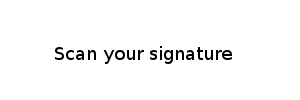
\includegraphics[height=1.5cm]{images/signature.png}

\vspace{1.5cm}

%%For the supervisor: Please type in your fullname according to the order given and include your electronic signature here%%
Supervisor: Firstname Middlename Surname 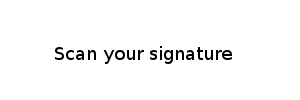
\includegraphics[height=1.5cm]{images/signature1.png}


\newpage

\chapter*{ACKNOWLEDGEMENTS}
\addcontentsline{toc}{chapter}{Acknowledgements}
% Don't change anything above this.
% We do not number this or add it to the contents!
% Overly long acknowledgements are not professional.

This is optional and should be at most half a page.
Thanks Ma, Thanks Pa. One paragraph in normal language is the most respectful.  

Do not use too much bold, any figures, or sign at the bottom.
\newpage
\chapter*{DEDICATION} 
\addcontentsline{toc}{chapter}{Dedication}

This is optional.

% Abstracts are usually written in English, with a version in your
% mother tongue underneath
\chapter*{Abstract} 
\addcontentsline{toc}{chapter}{Abstract}
% Don't change anything above this.

A short, abstracted description of your essay goes here. 
It should be about 100 words long. But write it last.

An abstract is not a summary of your essay: it's an abstraction of that. 
It tells the readers why they should be interested in your essay but summarises all
they need to know if they read no further.

The writing style used in an abstract is like the style used in the rest of your essay: concise, clear and direct. 
In the rest of the essay, however, you will introduce and use technical terms. In the abstract you should
avoid them in order to make the result comprehensible to all.

You may like to repeat the abstract in your mother tongue.

% At a unviersity like Stellenbosch you *must* produce an abstract in Afrikaans for your masters.
% At AIMS you are encouraged to repeat the abstract in your mother tongue
% French, Igbo, Mlagasy, etc. just write it using LaTeX's special
% characters.
% Arabic students see the arabic.tex file for an example
% Amharic use openoffice and export from there and import a figure here.
% Where the words do not exist put the English work in italics, or use mathematical symbols.





% Don't go typing out the contents.
\tableofcontents
\newpage
% We switch to arabic numerals here where your page count starts
% Essays must be 35 pages long *starting here* and up to and including
% the conclcusion. It does not include the acknowledgements or references.
% 
% Figures may differ between topics, but they are not there
% to fill the pages -- they must add meaning.
% In general most figures should be 0.8 times the width of the page
% (perhaps wider in total when two or three columns of figures)
% See the example in chapter one for defining that. Be *consistent*
% in your presentation of information.
\pagenumbering{arabic}
\pagestyle{myheadings}
%-----------------------------------------------------------------------------
% Each chapter goes in a separate file
% Chapter titles are just examples
% Always have a question
% Note the Case Pattern used at AIMS
\chapter{Introduction}

\section{Problem Statement}

%Explain the context of your essay topic, so that the
%topic itself appears motivated, natural and important.


%Paragraphs are separated by blank lines in the \LaTeX\ code, 
%and the line spacing, paragraph indentation,
%and paragraph spacing are set in the preamble for you, 
%according to AIMS house style.

%This is a textual citation \citet{shannon44}. And this is a parenthetical citation \citep{shannon44}. You probably want to use the latter more often.

%\begin{figure}[h]
%\psfrag{A}{$d^2$}
%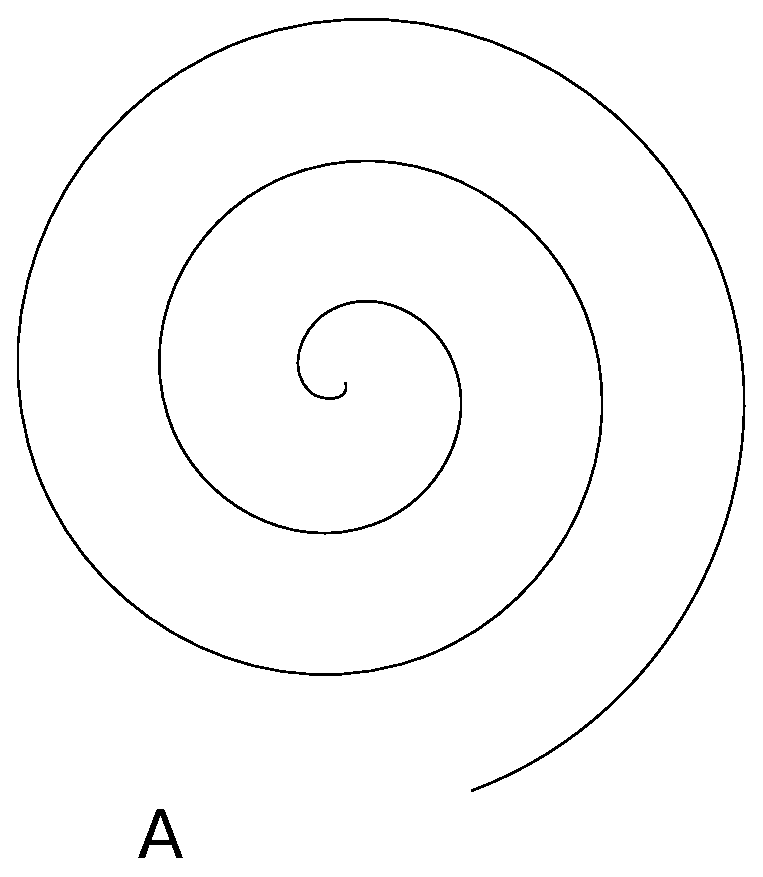
\includegraphics[scale=0.5]{images/drawing.eps}
%\end{figure}

Risk management is one of the fundamental tasks of insurance companies. The insurance industry should constantly adopt new technologies to address new risk types and trends affecting peoples lives.We depend on insurance for several reasons but it all scales down to the basic principle: minimizing risk in that clients pay a fee, and in exchange, insurers cover any costs that could arise with future calamities.

Clients provide extensive information to identify risk classification and illegibility, including scheduling medical exams, family medical history, credit history, behavioural risk factors, and so on, making the whole insurance process lengthy.The outcome is that the clients are turned off.This constitutes the main reason why majority of the households do not own individual life insurance.

Life underwriting has its own modelling challenges making insurers to turn to predictive  analytics to curb the problems.It is worth noting that auto underwriting has achieved remarkable success with predictive modelling unlike life underwriting where modelling is a new skill \citep{MikeBatty}. 

Building a predictive model requires:

\begin{enumerate}
\item[•] The availability of a sufficiently rich dataset where the predictive variables  correlate with the target can be identified

\item[•] An application by which results from the model are translated to business actions

\item[•] A clearly defined target variable

\item[•] A large number of observations to build the model so as surfacing relationships can be separated from random noise
\end{enumerate}

The above requirements are easily met with auto insurance.To clearly understand the challenges faced in life insurance, we compare life underwriting and auto underwriting.

\begin{enumerate}

\item[•] Auto insurers can make underwriting corrections if mistakes are made through rate increases in subsequent renewals of policies whereas life insurers must price policies appropriately from the outset

\item[•] For the auto insurer, the amount of insurance loss of a six-month contract is a target variable for the model. Life insurance is sold through long duration contracts, usually over a period of 10, 20 or more years.Due to the fact that the contribution of a given risk factor to mortality could change with time, it is not sufficient to analyse mortality experience over a short period of time

\item[•] Accessing historical data that can be used in modelling life insurance is a challenge.Not all life insurers record underwriting data in an electronic format; The available underwriting data that has been implemented in recent years is not available electronically or in a machine readable form. Even when such data has been captured for years, the content of the older data may be different from the data gathered for current applicants

\item[•] Life underwriting is subject to psychological biases and inconsistencies of human decision-making thus predictive models help to curb this challenge

\item[•] Life insurance claims have low frequency compared to auto insurance claims. Modelling statistically significant variation in either auto claims or mortality requires a large sample of loss events. Therefore auto insurers have ample data to build robust models using loss data while life insurers will find the data recorded in at similar times frames insufficient for modelling

Given that the target variable and data volume in life insurance is a concern, insurers are utilizing underwriting decisions as the target variable as they contain a lot of information, expert judgement, do not require long developing periods as in insurance claims and are abundant in supply.
\end{enumerate}

\section{Objective}
I am working on data from Prudential Life Insurance where the challenge is trying to make purchasing of life insurance easier by developing a predictive model that accurately classifies risk using a more automated approach. The data i am working on is from kaggle which is a platform for data science competitions. The host provides raw data and a description of the problem. Those participating in the competition then train algorithms where highly performing models can be adopted for predicting similar trends in the future.

\section{Trends in Insurance}
%Let's demonstrate a figure by looking at Fig.~\ref{bandwidth}. 
%
%\begin{figure}[!h]
% Use "\centering" in floats (figure, table), but if you need to center
% some text (why?) use "\begin{center}...\end{center}".
%\centering 
% Figure environments same as 0.8 * \textwidth please
% That does not necessarily mean the actual picture size,
% it is a guideline for the environmaRemember how to include code with {\tt verbatim} 
%and to fix the tabs in {\sf python} in a verbatim environment? 
%It may be best to have an `include' command for code, 
%not to have to re-edit it all the time.
%\verbatimtabinput{code/mycode.py}ndent which could contain
% 2 or more pictures! Be consistent and follow the guidelines
% provided in your sources.
%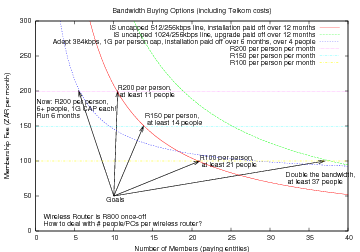
\includegraphics[width=0.8\textwidth]{images/bandwidth-colour.png}
%\caption{Planning community bandwidth sharing costs. 
%  Note caption capitalization.}
%\label{bandwidth} 
% if you move the label it breaks the reference numbering; 
% always have it *after* the caption.
%\end{figure}
 
%Remember how to include code with {\tt verbatim} 
%and to fix the tabs in {\sf python} in a verbatim environment? 
%It may be best to have an `include' command for code, 
%not to have to re-edit it all the time.
%\verbatimtabinput{code/mycode.py}

\textbf{Underwriting}

This is the process of understanding and evaluating risk in insuring a life or property.This ability is gained not only through theoretical study but also as a result of years of experience dealing with similar risks and mastering the art of paying claims on those risks. It is the traditional way of pricing and classifying risks in insurance \citep{macedo2009role}.

\citep{dickson2013actuarial} An insurance life office will have a premium rate schedule for a given type of policy.This rates depend on \textbf{the size of the policy and rating factors}.To establish an applicants risk level, a proposal form giving information on relevant rating factors such as age, gender,  any dangerous hobbies, occupation, smoking habits, and health history is filled. The purpose of underwriting is to classify potential policy holders into homogeneous risk categories and assess what additional premium would be appropriate if risk factors indicate that standard premium rates would be too low.


\textbf{Disadvantages}
\begin{enumerate}
\item[•] There is the risk of \textbf{adverse selection} by policy holders if the underwriting is not strict. This means that very high-risk individuals will buy insurance in disproportionate numbers leading to excessive losses.

\item[•] The underwriting process could be lengthy and costly

\item[•] Both the insurer and policy holder may assume 'utmost good faith' such that in case of loss and important information was held back or false,then the full sum assured may not be paid by the insurer in case the client claims from the insurance.
\end{enumerate}

Thus, the use of predictive models makes the underwriting process faster, more economical, more efficient and more consistent when the model is used to analyze a set of underwriting requirements.It is also worth noting that models are not subject to bias in the same way that underwriters ,who do not always act with perfect consistency or optimally weigh disparate pieces of evidence, are.

\section{Overview of Predictive Modelling}

In predictive modelling, two situations arise:

\begin{enumerate}
\item[•] One is required to fit a well-defined parametrized model to the data using a learning algorithm that can find parameters on the large dataset without over-fitting. In this case, lasso and elastic-net regularized generalised linear models are a set of modern algorithms which meet this need because they are fast, work on huge datasets and avoid over-fitting automatically.

\item[•] One needs to accurately predict a dependent variable. A learning algorithm that automatically identifies the structures, interactions and relationships in the data is needed. In this case, ensembles of decision trees (known as 'Random Forests') have been the most successful algorithm in modern times and basically this is what my work entails.
\end{enumerate}

\citep{berry1997data} Learning problems can be roughly categorized as either supervised or unsupervised.

\textbf{Supervised learning}: For each observation of the predictor measurement(s) $x_{i},i=1,2,...,n$, there is an associated response measurement $y_{i}$. We wish to find a model that relates the response to the predictors, with the aim of accurately predicting the response for future observations(predictions) and understand the relationship between the response and the predictors.Traditional statistical learning methods such as linear regression and logistic regression as well as modern approaches such as boosting and support vector machines work in the supervised learning domain.

\textbf{Unsupervised learning}: For every observation $i=1,2,...,n$, we observe a vector of measurements $x_{i}$ but no associated response $y_{i}$. A linear regression model cannot be fit because there is no response variable to predict.In this case we seek to find the relationship between the variables. One statistical tool that can be used is cluster analysis. Clustering ascertains whether the observations fall into distinct groups.

Supervised learning can be grouped into \textbf{Regression} and \textbf{Classification} problems.)

\begin{center}
\textbf{Regression Vs Classification Problems}
\end{center}
Variables can be grouped into \textbf{quantitative} or \textbf{qualitative} or categorical. Quantitative variables take on numerical values eg height while qualitative variables take on values in one of the different classes eg gender.

Problems with a quantitative response are referred to as regression problems while those involving a qualitative response are referred to as classification problems. Predicting a qualitative response for an observation is called classifying the observation since it involves assigning the observation to a class. Three of the most widely-used classifiers: logistic regression, k-nearest neighbors and Linear Discriminant Analysis. More computer-intensive methods are trees, random forests, support vector machines and boosting \citep{james2014introduction}.

\textbf{Machine Learning}: This is a method of teaching computers to improve and make predictions based on data.It is teaching a program to react to and recognize patterns through analysis, self training, observation and experience.

In the classification setting, we have a set of training observations $(x_{1},y_{1}),...,(x_{n},y_{n})$ that we can use to build a classifier. We want our classifier to perform well not only on the training data, but also on test observation not used to train the classifier.Here, I introduce some of the most commonly used classifiers.

\begin{center}
\textbf{Logistic Regression}
\end{center}

Models the probability that $Y$, the dependent variable belongs to a particular category (one of two categories eg 'yes' or 'no').


\textbf{The model}

Modelling the relationship between $p(X)=pr(Y=1/X)$ and $X$. For convenience we use the generic coding 0 and 1 for the response. To use linear regression to represent this probabilities we have, $p(X)=\beta_{0}+\beta_{1}X$ which gives the left hand side of the logistic function. 

However,there is a problem with this approach in that predicting of values close to zero would yield negative probabilities and if we were to predict large values, we would get probabilities bigger than 1 which defies the law of probability that probability values should fall between 0 and 1.

To prevent this,we model $p(X)$ using the logistic function that gives outputs between 0 and 1 for all values of $X$. 

\begin{equation*}
p(X)=\dfrac{\exp(\beta_0+\beta_{1}X)}{1+\exp(\beta_0+\beta_{1}X)}
\end{equation*}

We notice that for lower values, we now predict the probability of default as close to but never below $0$. Likewise for high values, we predict a default probability close to but, never above one.

Manipulating the equation gives;

\begin{equation}
\dfrac{p(X)}{1-p(X)}=\exp (\beta _0+\beta_{1}X)
\end{equation}

where the LHS is called odds and takes values between $0$ and $\infty$. Taking the logarithms on both sides yields:

\begin{equation}
log \left(\dfrac{p(X)}{1-p(X)}\right)=\beta_{0}+\beta_{1}X
\end{equation}

The LHS is called the log-odds or logit which is linear in $X$.

\begin{center}
\textbf{K-nearest Neighbors}
\end{center}

KNN can handle both binary and multi-class data.

Consider having $N$ training objects, each of which is represented by a set of attributes $X_{n}$ and a label $Y_{n}$.Suppose we want to classify new objects $X_{new}$, We first find the K training points closest to $X_{new}$. $Y_{new}$ is then set to be the majority class amongst these neighbors.

The figure below provides an illustrative example of the KNN approach \citep{james2014introduction}.

\begin{figure}[hbtp]
\caption{KNN approach using K=3.}
\centering
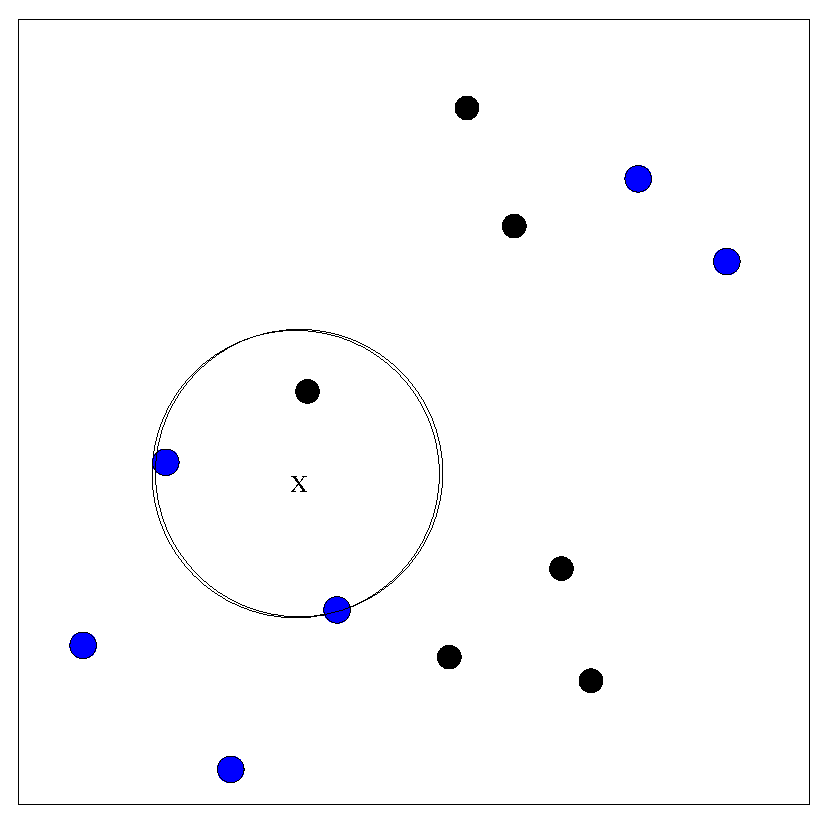
\includegraphics[scale=0.4]{KNN.eps}
\end{figure}


The goal is to predict the point labelled $X$. Suppose we choose $K=3$, KNN will first identify the three observations closest to $X$, as shown in the diagram. The point consists of two blue points and a red point resulting in estimated probabilities of $\dfrac{2}{3}$ for the blue class and $\dfrac{1}{3}$ for the black class. KNN will predict that the point $X$ belongs to the blue class.

\textbf{One draw back of KNN is the issue of ties}: Two or more classes having equal number of ties. Therefore,for binary classification,a good solution is to always use an odd number of neighbors.

\textbf{Choosing K}: If K is too small, the classification is heavily influenced by mislabelled points(noise). This problem is rectified by increasing K which regularises the boundary.

What about if K is too big? As we increase K, we are using neighbours further away from $X_{new}$ which is useful upto a certain point as it has a regularizing effect that reduces the chances of over-fitting.However, when we go too far, we loose the true pattern of the data we are attempting to model.Therefore, to find the best value of K, we use cross validation.

\begin{center}
\textbf{Linear Discriminant Analysis}
\end{center}

Linear Discriminant Analysis is used:
\begin{enumerate}
%\item[•] The parameter estimates for the logistic regression model are stable when the classes are well separated. LDA does not suffer from this problem.

\item[•] LDA is popular when we have more than two response classes.
\end{enumerate}

\textbf{Using bayes' theorem for classification}

Suppose we wish to classify an observation into K classes, where $K\geqslant 2$ and the qualitative response variable $Y$ can take on K distinct ordered values.

$\pi_{k}$: Denotes the prior probability that a randomly chosen observation comes from  class K of the response variable $Y$.

$f_{k}=Pr(X=x/Y=k)$: Denote the density function of X for an observation from class K.

Bayes theorem states that:

\begin{equation}
P_{k}(X)=Pr(Y=k/X=x)=\dfrac{\pi_{k}f_{k}(x)}{\sum \pi_{i}f_{i}(x)} \label{1.3.3}
\end{equation} 

$P_{k}(x)$: Posterior probability that an observation $X=x$ belongs to class K.

$\pi_{k}$ is computed if we have a random sample of $Y_{s}$ from the population. We therefore compute the fraction of training observations that belong to class K.$f_{k}(x)$ is estimated so we can develop a classifier that approximates the bayes classifier.

\begin{center}
Linear Discriminant Analysis for $p=1$.(We  have only one predictor)
\end{center}

We are required to find an estimate for $f_{k}(x)$ that we can plug into \eqref{1.3.3} inorder to estimate $p_{k}(x)$. We then classify an observation to the for which $p_{k}(x)$ is greatest. To estimate $f_{k}(x)$ the following assumptions are made:

\begin{enumerate}
\item[•] $f_{k}(x)$ is normal.
\begin{equation}
f_{k}(x)=\dfrac{1}{\sqrt{2 \pi}\sigma_{k}} \exp \left(-\dfrac{1}{2 \sigma^2_{k}}(x-\mu_{k})^2\right) \label{1.3.4}
\end{equation}

$\mu_{k}$ and $\sigma_{k}^2$ are the mean and variance parameters for class k.

\item[•] Shared variance term across all K classes, $\sigma_{1}^2=,...,=\sigma_{K}^2$
\end{enumerate}

Plugging equation \eqref{1.3.4} to equation \eqref{1.3.3} yields:

\begin{equation}
p_{k}(x)=\dfrac{\pi_{k}\dfrac{1}{\sqrt{2 \pi}\sigma} \exp \left(-\dfrac{1}{2 \sigma^2}(x-\mu_{k})^2\right)}{\sum_{i=1}^{K} \pi_{i}\dfrac{1}{\sqrt{2 \pi}\sigma} \exp \left(-\dfrac{1}{2 \sigma^2}(x-\mu_{i})^2\right)} \label{1.3.5}
\end{equation}

Taking the logs of equation \eqref{1.3.5} and rearranging the terms gives:

\begin{equation}
\delta_{k}(x)=x \dfrac{\mu_{k}}{\sigma^2}-\dfrac{\mu^2_{k}}{2 \sigma^2}+log(\pi_k) \label{1.3.6}
\end{equation}

It is not possible to calculate the bayes  classifier in real-life. We still need to estimate the parameters $\mu_{1},...,\mu_{K}, \pi_{1},...,\pi_{K}$ and $\sigma^2$. LDA method approximates the bayes classifier by plugging the estimates for $\pi_{k}, \mu_{k}$ and $\sigma^2$ into equation \eqref{1.3.6}.

The following estimates are used:

\begin{align}
\hat{\mu_k}&=\dfrac{1}{n_{k}} \sum _{i:y_i=k} x_{i}\\ \label{1.3.7}
\hat{\sigma}&=\dfrac{1}{n-K} \sum _{K=1}^K \sum _{i:y_i=k}(x_{i}-\hat{\mu})^2\\ \label{1.3.8}
\end{align}

$n$: Number of training observations
$n_k$: Total number of training observations in class k where $\mu_k$ is the average of all training observations from class k.

$\hat{\sigma}^2$: Weighted average of the sample variances for each of the k classes.

In the case where additional information is not present, LDA estimates $\pi_{k}$ using the proportion of training observations that belongs to the $k^{th}$ class.

\begin{equation}
\pi_{k}=\dfrac{n_k}{n} \label{1.3.9}
\end{equation}

LDA classifier plugs the estimates equation \eqref{1.3.7} and equation \eqref{1.3.8} into equation \eqref{1.3.6}, assigning an observation $X=x$ to the class for which 

\begin{equation}
\hat{\delta}_{k}(x)=x \dfrac{\hat{\mu_{k}}}{\hat{\sigma}^2}-\dfrac{\hat{\mu}^2_{k}}{2 \hat{\sigma}^2}+log(\hat{\pi}_k)
\end{equation}
is largest.

The classifier is linear due to the fact that the discriminant functions $\hat{\delta}_{k}(x)$ are linear functions of $x$.

I will use random forest for my analysis which i will discuss in depth in the subsequent chapter. % Introduction is usually a chapter itself.
\chapter{The Second Chapter}
\section*{Methodology}
Random forests are a combination of tree predictors such that each tree depends on the values of a random vector sampled independently and with the same distribution for all trees in the forest(Breiman,2001).The goal of Random forest is creating a predictive model that predicts the value of a target variable bbased on given input variables where one of the input variable is represented by each interior node and the values of the input variable is represented by edges.

\begin{center}
\textbf{Bagging and Random forests}
\end{center}
 
Bagging and random forests use trees as building blocks to constructing more powerful models.

\textbf{Bootstrap}: It is a widely used statistical tool used to quantify uncertainty associated with given estimators. It can easily be applied to a wide range of statistical learning methods even those whose measure of variability is difficult to obtain.

\textbf{Bootstrap aggregation / Bagging}: This is the basic principle behind the training algorithm for random forests which reduces the variance of a statistical learning method.

Consider the set of $n$ independent observations denoted by $C_1,C_2,...,C_3$ each with variance $\sigma^2$. Therefore the variance of the mean $\bar{Z}$ of the observation is given by $\dfrac{\sigma^2}{n}$. Averaging a set of observations reduces the variance.To reduce the variance and increase the prediction accuracy of a statistical learning method, we sample many training sets from the population,build a separate prediction model and average the resulting predictions. Therefore, calculate $\hat{f}^{1}(x),\hat{f}^{2}(x),...,\hat{f}^{B}(x)$ using $B$ separate training sets and average them so as to obtain a single low-variance statistical model given as:

\begin{equation}
\hat{f}_{avg}(x)=\dfrac{1}{B} \sum_{b=1}^{B} \hat{f}^{b}(x)
\end{equation}

However, this is not practical because we cannot have multiple training sets so the bootstrap approach is used where repeated samples from the single training dataset are sampled.In this method, $B$ different bootstrapped training datasets are generated and we train our method on the $b^{th}$ bootstrapped training set to obtain $\hat{f}^{\star b}(x)$ and then average all the predictions to obtain:

\begin{equation}
\hat{f}_{bag}(x)=\dfrac{1}{B} \sum_{b=1}^{B} \hat{f}^{\star b}(x)
\end{equation}

This is called \textbf{bagging}. (When trees are repeatedly fit to bootstrapped subsets of the observations)

So given a training set $X=x_1,...,x_2$ with responses $Y=y_1,...,y_n$, bagging repeats $B$ times and selects random samples \textbf{with replacement} of the training set and fits trees to the sample.Trees are grown deep and are not pruned therefore each individual tree has high variance but low bias.Finding the average of the $B$ trees reduces the variance.

\textbf{How can bagging be extended to a classification problem where $Y$ is qualitative?} Given a test observation, a predicted class can be recorded by each of the $B$ trees and a majority vote is recorded. The overall prediction is the most commonly occurring class among the $B$ predictions.

\begin{center}
\textbf{Out of Bag Error Estimation}
\end{center}

This is a method of estimating the test error of a bagged model without the need of cross validation. Averagely, each bagged tree makes use of around $\dfrac{2}{3}$ of the observation and the other $\dfrac{1}{3}$ of the observation is not used to fit a bagged tree. This observations are referred to as out of bag observation. The response for the $i^th$ observation can be predicted using each of the tree in which that observation was out of bag which will yield around  $\dfrac{B}{3}$ predictions for the $i^th$ observation. To obtain a single prediction for the $i^th$ observation,we take a majority vote of the predicted responses. This gives a single OOB prediction for the $i^th$ observation.

The OOB prediction is obtained for the $n$ observations and the classification error is computed.The OOB error is an estimate for the test error for the bagged model since each of the observation has the response predicted using only the trees that were not fit using that observation. Therefore, the OOB method for test error estimation is convenient when bagging on large datasets. 

%QUOTE HERE
For each observation $Z_{i}=(x_{i},y_{i})$ we build a random forest predictor by averaging the trees corresponding to bootstrap samples in which $z_{i}$ did not appear. The training is terminated when the error stabilizes.

\begin{center}
\textbf{Variable importance measures}
\end{center}

When a large number of trees are bagged, it is no longer possible to represent the statistical learning procedure using a single tree,and it is not also clear which variables are most important to the procedure. Although the collection of bagged trees is difficult to interpret than a single tree, an overall summary of the importance of each predictor can be obtained using the gini index for bagging classification trees.

\textbf{Gini index}: This is the expected error rate of the system.Calculating the gini index for each attribute helps one to get the splitting attributes.


\begin{center}
\textbf{Random Forests}
\end{center}

Random forest is an improvement over bagged trees by providing a small adjustment to the system that decorrelates the trees. In building the decision trees, \textbf{a random sample of m predictors is chosen as split candidates from the set of p predictors} each time a split in a tree is considered. The split is allowed to use only one of those m predictors.

The number of predictors considered at each split is approximately equal to the square root of the total number of predictors, $m\approx \sqrt{p}$. A new sample of $m$ predictors is taken at each split.

Suppose there is one very strong predictor in the dataset and a number of other moderately strong predictors. Then most or all of the predictors will use the strong predictors in the top split in the collection of the bagged trees. Consequently,
all of the bagged trees will look quite similar to each other and therefore the predictions from the bagged trees will be highly uncorrelated. Bagging will not lead to a reduction in the variance over a single tree in this setting.

\textbf{How does random forest overcome this problem?} By ensuring that each split considers only a subset of the predictors.Averagely, $\dfrac{(p-m)}{p}$ of the splits will not consider the strong predictorand the other predictors will have a chance.This is referred to as \textbf{decorrelating the trees}. This approach makes the average of the resulting trees less variable and more reliable.

\textbf{The main difference between bagging and Random Forest} is the choice of the predictor subset size $m$. If a random forest is built using $m=p$, this amounts to bagging. Random Forest using $m=\sqrt{p}$ leads to a reduction in \textbf{test error} and \textbf{OOB} over the bagging technique. It is helpful to use a small value of $m$ when building a random forest if we have a large number of uncorrelated predictors.Random forest does not overfit just like bagging if we increase B.

\begin{center}
\textbf{Implementing the Random forest algorithm}
\end{center}

%\textbf{Data Exploration}.
\begin{enumerate}
\item[•] Loading the Data: The code loads the train(rawdata1) and test(test2) data into the jupyter notebook. The scope of the project is to predict the feature response which are the different categories of risk in the test data.

\begin{verbatim}
raw_data1=pd.read_csv('train.csv')  #loading the train data
test2=pd.read_csv('test.csv')  #loading the test data
\end{verbatim}

\item[•] Shape of the data: The train data is composed of 59,381 observations and 128 features while the test data is composed of 19765 observations and 127 features.

\begin{verbatim}
raw_data1.shape
(59381, 128)
\end{verbatim}

\begin{verbatim}
test2.shape
(19765, 127)
\end{verbatim}

\item[•] To list the features in the data:
\begin{verbatim}
raw_data1.columns.values
\end{verbatim}

\item[•] Factorize string variable: Product Info 2 is a string categorical variable, we transform this feature to enumerate type using the factorize function.The factorize functions returns a list of unique values (or categorical labels) in the product Info 2 column.
\begin{verbatim}
raw_data['Product_Info_2'] = pd.factorize(raw_data['Product_Info_2'])[0]  
raw_data['Product_Info_2']
\end{verbatim}

\item[•] Missing values: From sklearn we import imputer. Where the missing values is Nan, we choose the imputation strategy as mean and the axis is set to 0 meaning that we want to impute the mean values along the columns. The strategy can also be mode incase we replacing categorical missing values. We therefore choose the most occurring value or the median value along the axes.
\begin{verbatim}
imp=Imputer(missing_values='NaN', strategy='mean', axis=0)
imp.fit_transform(raw_data,y='Response')
\end{verbatim}

\item[•] Splitting the data into into train and test.

From sklearn we import model selection which splits the dataset into random train and test subsets.

Test size: Gives the proportion of the dataset that is included in the test split.

Random state: Pseudo-random number generator state that is used for random sampling. 

\begin{verbatim}
train_raw, test_raw=model_selection.train_test_split(raw_data,
test_size=0.4, random_state=100)
\end{verbatim}

\item[•] To prepare the data for modelling, we drop the features 'Id' and 'Response'.

\begin{verbatim}
t1=train_raw.drop(0,axis=1)    #Train_raw dataset
t2= test_raw.drop(0,axis=1)     #Test_raw dataset
t1=t1.drop(127,axis=1)
t2=t2.drop(127,axis=1)
\end{verbatim}

\item[•] Assigning the response and explanatory variables to numpy array.


\begin{verbatim}
ob=list(t1.columns)
def choose_columns(data):
    ret_X= np.array(data.loc[:,ob]) #Explanatory variables
    ret_Y=data.values[:,-1]
    return ret_X, ret_
\end{verbatim}

\item[•] We model the data using the Random Forest algorithm.

From sklearn.ensemble we import the RandomForestClassifier.

\begin{verbatim}
import sklearn.ensemble as en
RF= en.RandomForestClassifier(n_estimators= 250, criterion='gini',
   max_depth=None,min_samples_split=2, min_samples_leaf=1,max_features='auto',   
   max_leaf_nodes=None, min_impurity_split=1e-08,bootstrap=True,            
   oob_score=False,n_jobs=1, random_state=None, verbose=0,warm_start=True)
\end{verbatim}
Description of the parameters that i tuned for the best score.

n\_estimators: The number of trees in the forest.

Criterion: "gini", measures the quality of a split.

max\_depth: The maximum depth of the tree.Takes on integer values or none.If the value is none, then all nodes are expanded until all leaves are pure.

Min\_samples\_split: Minimum number of samples required to split an internal node.

Min\_samples\_leaf: The minimum number of samples required to split an internal node.

Max\_features: Number of features to consider when looking for the best split. If it is auto, then the max features is equal to the sqrt(n features).

Max\_leaf\_nodes: This parameter grows trees with max leaf nodes in the best first fashion.

Min\_impurity\_split: This is the threshold for early stopping in the tree growth. A node will split if its impurity is above the threshold, otherwise it is a leaf.

Bootstrap: It takes on boolean with default =True. If true, the algorithm makes use of bootstrap samples when building the trees.

Oob\_score: It takes on boolean with default =True. If true, the algorithm uses the out of bag samples to estimate the generalization accuracy.

n\_jobs: Default=1. The number of jobs that should run in parallel for bothfit and predict. If -1, then the number of jobs is set to the number of cores.

Random state: If none, it means that the random number generator is the random state instance  used by np.random.

Verbose: Default=0. Controls the verbosity of the tree building process. That is if the verbose is set to a higher number, more information about the tree building process will be seen.

Warm\_start: bool,(default=False). When set to true,the solution of the previous call to fit and add more estimators to the ensemble is reused. Otherwise, just fit a whole new forest.

\item[•] Fit the Random Forest classifier on the train data.

\item[•] Then predict the response feature for the test data that was split using the model selection code. 

\item[•] The same feature transformations are done on the test data provided by kaggle. This is the data we are supposed to predict the response variable and evaluate the score using the quadratic weighted kappa metric.
\end{enumerate}
 \textbf{Quadratic weighted kappa metric}: It can be used to quantify the amount of agreement between the predictions from an algorithm and some trusted labels of the same objects in machine learning. It is a chance adjusted index of agreement and measures the agreement between two ratings.

Calculation of quadratic weighted kappa metric.
\begin{enumerate}
\item[•] We construct an $N\times N$ histogram matrix $O$.$O_{ij}$ corresponds to the number of applications which received a rating $i$ by A and $j$ by B.

\item[•] We calculate an $N\times N$ matrix of weights ,$w$, based on the difference between the rater's score.

\begin{equation}
w_{ij}=\dfrac{(i-j)^2}{(N-1)^2}
\end{equation}

\item[•] An $N\times N$ histogram matrix of expected ratings, E, is calculated, making the assumptions that there is no correlation between the rating scores. This is calculated as the outer product between each rater's histogram vector of ratings and normalized such that E and O have the same sum.

\item[•] The quadratic weighted kappa is calculated from these three matrices as:

\begin{equation}
\dfrac{1-\sum_{ij}w_{ij}o_{ij}}{\sum_{ij}w_{ij}E_{ij}}
\end{equation}

The metric works well for a highly imbalanced classification task. The metric varies from 0 (random agreement) to 1 (complete agreement).In case there is less agreement between the raters than expected by chance, this metric may go below 0. The data has 8 possible ratings and each application is characterized by a tuple (ea,eb), that corresponds to the scores by rater A, actual risk and rater B, predicted risk. 
\end{enumerate}

My predictions on kaggle scored \textbf{0.53074}.

\textbf{Weakness of Random forest}
\begin{enumerate}
\item[•] Random forest may overfit noisy datasets

\item[•] Having a large number of trees makes the algorithm slow for real time prediction
 
\end{enumerate}

To improve my score on kaggle, I employed the Xgboost algorithm whose full name is eXtreme Gradient Booosting. It is a variant of gradient boosting, which is a tree model based supervised learning algorithm. Unlike fitting a single large decision tree to the data, which could amount to overfitting, the boosting approach instead learns slowly. It includes an efficientlinear model solver and a tree learning algorithm.


\begin{center}
\textbf{Xgboost Algorithm}
\end{center}

The full name is eXtreme Gradient Boosting. It is a variant of gradient boosting, a tree model based supervised learning algorithm. It includes an efficient model solver and a tree learning algorithm. This boosting approach learns slowly unlike fitting a large decision tree to the data which likely amounts to overfitting the data.

\textbf{Features of Xgboost}
\begin{enumerate}
\item[•] Customization: Xgboost supports customized objective function and evaluation function.

\item[•] Sparcity: Xgboost accepts sparse input for both the tree andlinear booster, and is optimized for sparse input.

\item[•] Input type: Xgboost takes several types of input data. The recommended type is xgb.Dmatrix.

\item[•] Speed: It can automatically do parallel computation and faster than gradient boosting machine.

\item[•] Performance: Has better performance on different datasets.
\end{enumerate}

\textbf{XG Boost paramers}

The parameters can be grouped into:
\begin{enumerate}
\item[1] General parameters.

Under general parameters we have number of threads.

\item[2] Booster parameters.
\begin{itemize}
\item Stepsize
\item  Regularization
\end{itemize}
       
\item[3] Task parameters.

\begin{itemize}
\item[•] Objective
\item[•] Evaluation metric
\end{itemize}
\end{enumerate}

\begin{center}
\textbf{Model Specification}
\end{center}

%Take this section next to the code and continue with description of rest.
General parameters.
\begin{itemize}
\item nthread: Number of parallel threads.

\item Booster: 
  \begin{itemize}
  \item[•] gblinear: linear function.
  \item[•] gbtree: tree based model.
  \end{itemize}
\end{itemize}
%\textbf{Parameters for tree booster}

\textbf{Implementing the XGBoost algorithms}
\begin{enumerate}

\item[•] \begin{verbatim}
def eval_wrapper(yhat, y):  
    y = np.array(y)
    y = y.astype(int)
    yhat = np.array(yhat)
    yhat = np.clip(np.round(yhat), np.min(y), np.max(y)).astype(int)   
    return quadratic_weighted_kappa(yhat, y)
\end{verbatim}

This function calculates the quadratic weighted kappa metric.

np.clip: Takes three arguments (np.clip(a, a min, a max, out=None)). It clips (limits) the values in an array. Given an interval, values outside the interval are clipped to the interval edges.

np.round: (a,decimals=0,out=None). Evenly rounds to the given number of decimal places.

\item[•] \begin{verbatim}
def get_params():
    
    params = {}
    params["objective"] = "reg:linear"     
    params["eta"] = 0.05
    params["min_child_weight"] = 360
    params["subsample"] = 0.85
    params["colsample_bytree"] = 0.3
    params["silent"] = 1
    params["max_depth"] = 7
    plst = list(params.items())

    return plst
\end{verbatim}

This code sets up a dictionary of parameters for the tree booster.
Objective
\begin{itemize}
\item "reg:linear": default option, Linear regression.

\item "binary: Logistic": Outputs probability. It performs logistic regression for binary classification.

\item "multi:softmax": Uses the softmax objective for multiclass classification.
\end{itemize}

Eta/Learning rate: We can directly get weights of new features after each boosting step. Eta shrinks the feature weights and makes the boosting process more conservative.
Eta is the stepsize shrinkage used in update to prevent overfitting. It is in the range of [0,1], the default is 0.3.

Min\_child\_weight: This is the minimum sum of instance weight needed in a child. It ranges from [0,$\infty$] and the default is 1.

The tree building process will give up further partitioning if the tree partition step results in a leaf node with the sum of instance weight less than the Min\_child\_weight.

Subsample: It is the subsample ratio of the training instance. Setting it to 0.5 means that XGBoost randomly samples half of the data instances and grows trees thus prevents overfitting. It ranges from (0,1], the default value being 1. This parameter makes the model more robust and avoids overfitting.

colsample\_bytree: This is the subsample ratio of columns when constructing each tree. The range is (0,1] and the default is 1. Both subsample and colsample\_bytree cannot be set to 0.

Silent: The default=0. 0 means printing running messages, 1 means silent mode.

max\_depth: This is the maximum depth of a tree. Increasing the max\_depth value makes the model more complex and more likely to overfit. The range is from [1,$\infty$], the default is 6. 

\item[•] \begin{verbatim}
def score_offset(data, bin_offset, sv, scorer=eval_wrapper):
    # data has the format of pred=0, offset_pred=1, labels=2 in the first dim
    data[1, data[0].astype(int)==sv] = data[0, data[0].astype(int)==sv] +   
     bin_offset
    score = scorer(data[1], data[2])
    return score
\end{verbatim}
\end{enumerate}




\newpage
A plot of the feature importances lists the most important features in descending order.
 
\vspace{1pc}
\begin{figure}[hh!]
\caption{Feature Importance}
%\centering
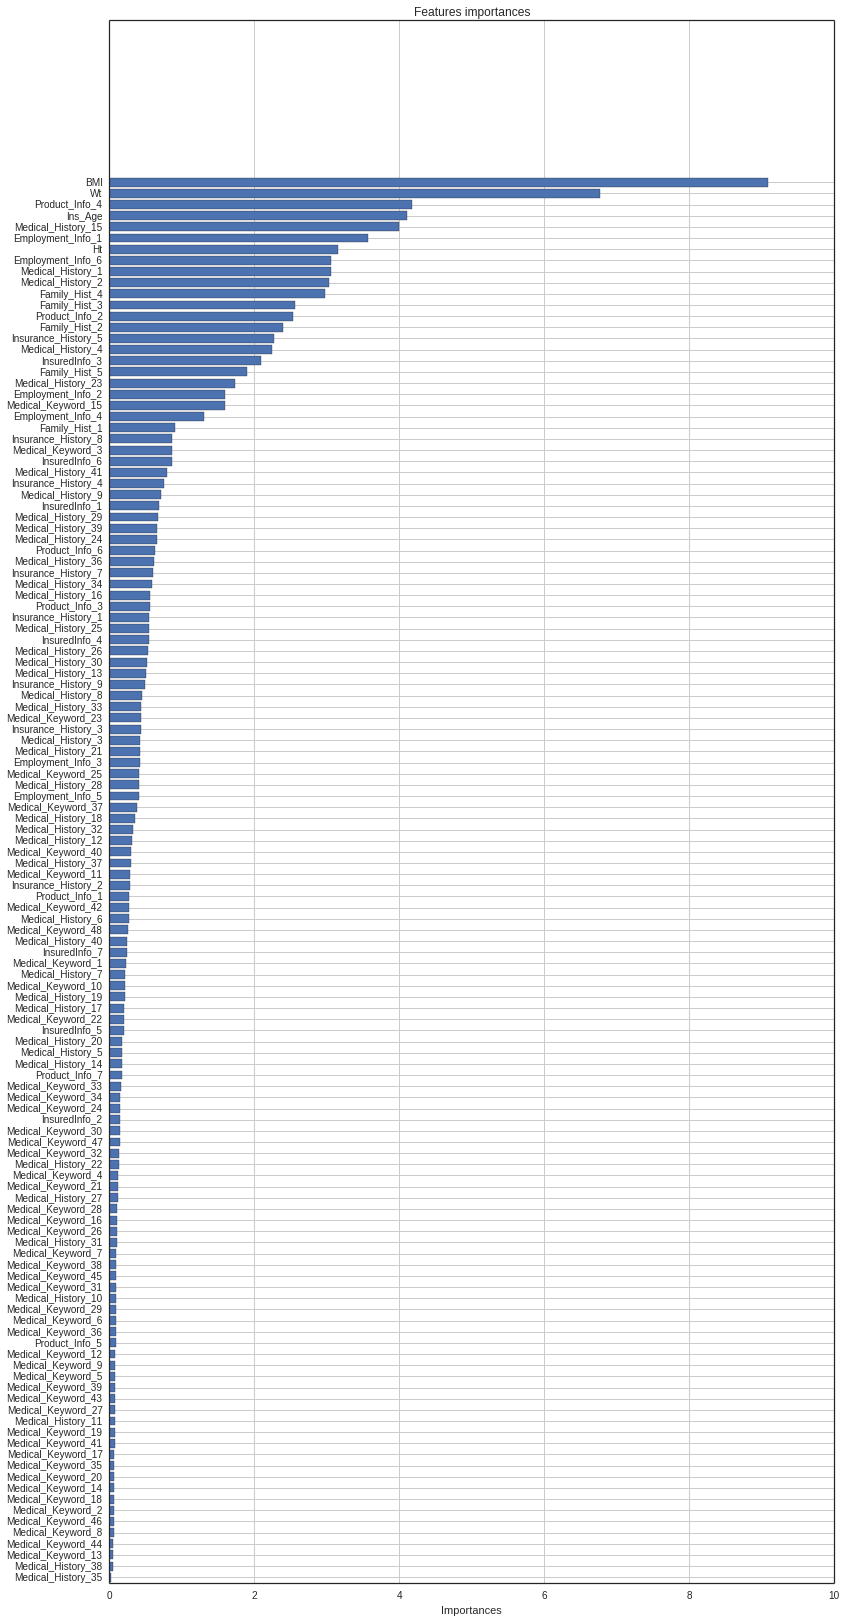
\includegraphics[scale=0.2]{index.png}
\end{figure}

The figure above is a variable importance plot for the insurance data.Variable importance is computed using the mean decrease in the gini index and expressed relative to the maximum.

The code below outputs the five most important and least important variables in ascending order respectively.

\begin{verbatim}
importances =pd.DataFrame({'features' :m.columns,
                           'importances' : RF.feature_importances_})
importances.sort_values(by='importances',ascending=False).head(5)
importances.sort_values(by='importances',ascending=False).tail(5)
\end{verbatim}

\begin{tabular}{|c|c|}
\hline 
\multicolumn{2}{|c|}{The first 5 important predictors} \\ 
\hline 
BMI & 0.089700 \\ 
\hline 
Wt & 0.068185 \\ 
\hline 
Product info 4 & 0.041591 \\ 
\hline 
Ins Age & 0.040372 \\ 
\hline 
Medical History & 0.039763 \\ 
\hline 
\multicolumn{2}{|c|}{The last 5 less important predictors} \\ 
\hline 
Medical History 35 & 0.000219\\
\hline 
Medical History 38 & 0.000512 \\ 
\hline 
Medical History 13 & 0.000551 \\ 
\hline 
Medical History 44 & 0.000612 \\ 
\hline 
Medical History 8 & 0.000622 \\ 
\hline 
\end{tabular} 

\begin{center}
\textbf{Data Visualization}
\end{center}

The scatter plot below shows the relationship between the various responses and the normalized Ins Age.

\begin{figure}[hbtp]
\caption{Scatter plot af Age Vs Response}
\centering
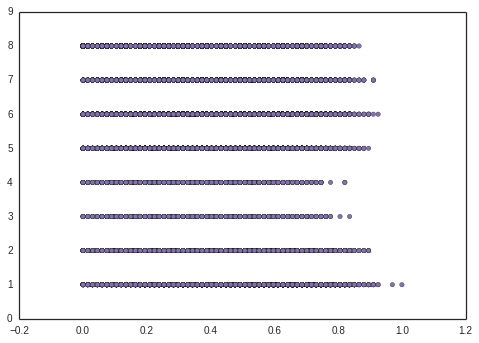
\includegraphics[scale=0.5]{Scatterplot.png}
\end{figure}

The response classes are imbalanced as shown in the plot below.

\begin{figure}[hbtp]
\caption{Class Imbalance of the response variable}
\centering
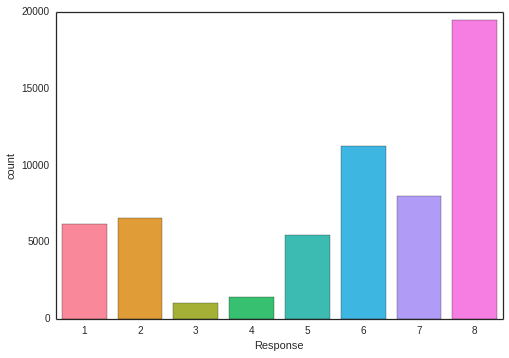
\includegraphics[scale=0.5]{classimbalance.png}
\end{figure}

Visualization of various feature plots.
\begin{figure}[hh!]
  \centering
  \begin{subfigure}[b]{0.4\textwidth}
     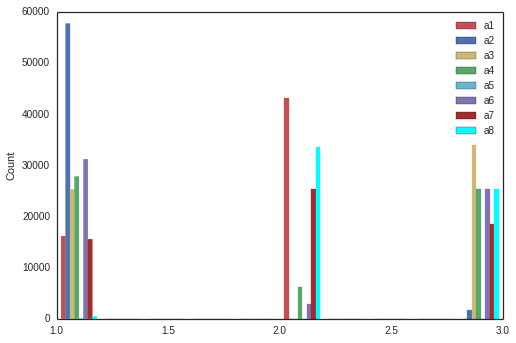
\includegraphics[width=\textwidth]{Insurancehist.png}
     \caption{Insurance history plot}
     \label{imbalance}
  \end{subfigure}
  \quad
   \begin{subfigure}[b]{0.4\textwidth}
      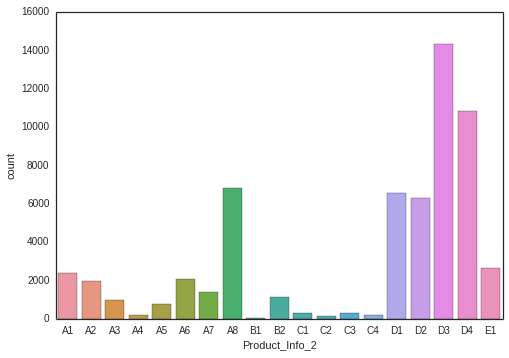
\includegraphics[width=\textwidth]{categoricalplot.png}
      \caption{Product Info 2}   
   \end{subfigure}
   \caption{Feature data plots}
\end{figure}

\begin{figure}[hh!]
  \centering
  \begin{subfigure}[b]{0.4\textwidth}
     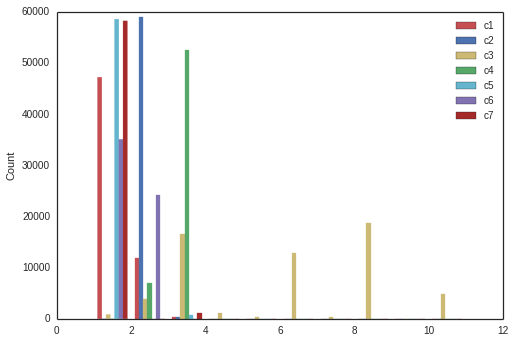
\includegraphics[width=\textwidth]{Insuranceinfo.png}
     \caption{Insurance information plot}
     \label{imbalance}
  \end{subfigure}
  \quad
   \begin{subfigure}[b]{0.4\textwidth}
      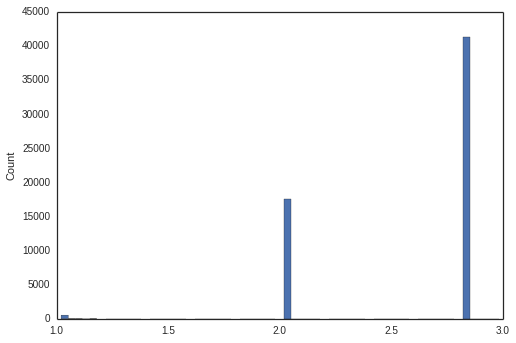
\includegraphics[width=\textwidth]{Familyhist.png}
      \caption{Family history plot}   
   \end{subfigure}
   \caption{Feature data plots}
\end{figure}

\begin{figure}[hh!]
  \centering
  \begin{subfigure}[b]{0.4\textwidth}
     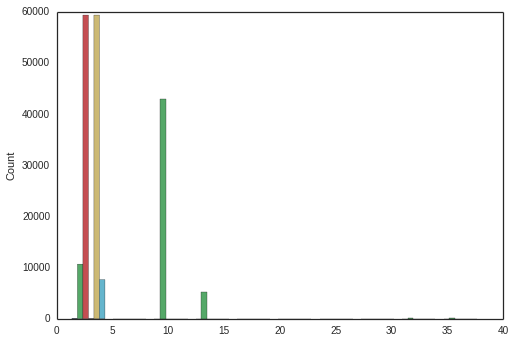
\includegraphics[width=\textwidth]{EmploymentInfo.png}
     \caption{Employment information plot}
     \label{imbalance}
  \end{subfigure}
  \quad
   \begin{subfigure}[b]{0.4\textwidth}
      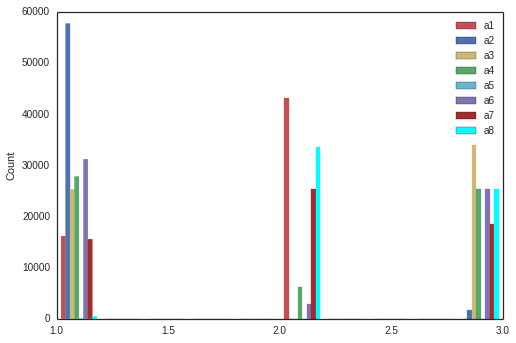
\includegraphics[width=\textwidth]{Insurancehist.png}
      \caption{Insurance history plot}   
   \end{subfigure}
   \caption{Feature data plots}
\end{figure}



%Text text text text text text text text text text text text text text
%text text text text text text text text text text text text text text.
%
%When you get stuck, don't panic. 
%The world is unlikely to end just now. 
%Remember you can consult your supervisor, tutor, and Blaise at agreed times. 
%
%\begin{thm}[Jeff's Washing Theorem]
%\label{thm:jwt}
%If an item of clothing is too big, then washing it makes it bigger;
%but if it is too small, washing it makes it smaller.
%\end{thm}
%\begin{proof}
%Stated without proof. But a proof would look like this. 
%\end{proof}
%
%Notice that no Lemmas are required in the proof of Theorem \ref{thm:jwt}.
 % Chapters might go from 2. problem statement, 
                 % through 3. model, to 4. analysis & results
\chapter{Third Chapter}

Theorems before the chapter's first section will be dot-zero, 
and their numbering is completely wrong. You can avoid this
by simply always starting a chapter with a section. Ta Da! 
It will probably help you structure your essay anyway. 

\begin{thm}[My Theorem2]
This is my theorem2.
\end{thm}
\begin{proof}
And it has no proof2.
\end{proof}

\section{See?}

Text text text text text text text text text text text text text text
text text text text text text text text text text text text text text
text text text text text text text text text text text text text text
text text text text text text text text text text text text text text
text text text text text.

\begin{thm}[My Theorem2]
This is my theorem2.
\end{thm}
\begin{proof}
And it has no proof2.
\end{proof}

Text text text text text text text text text text text text text text
text text text text text text text text text text text text text text
text text text text text text text text text text text text text text
text text text text text text text text text text text text text text
text text text text text.

\begin{align} % do not use eqnarray. 
\label{2ya}
x & = y + y\\
\label{2yb}
& = 2y
\end{align}
see equations \eqref{2ya} and \ref{2yb}

\section{More}

Here's a conjecture
\begin{conj}
The washing operation has fixed points.
\end{conj}

and here's an example

\begin{exa}
100 FRW coin.
\end{exa}

\subsection{This is a subsection}

\section{This is a section}
 % You do not need to have exactly 4 chapters.
                 % It is probably a good minimum, with 5 chapters 
                 % average, and 7 chapters might be a maximum.
\chapter{The Second Squared Chapter}

An average essay may contain five chapters, but I didn't plan my work properly
and then ran out of time. I spent too much time positioning my figures and worrying
about my preferred typographic style, rather than just using what was provided.
I wasted days bolding section headings and using double slash line endings, and 
had to remove them all again. I spent sleepless nights configuring manually numbered lists
to use the \LaTeX\ environments because I didn't use them from the start or understand
how to search and replace easily with texmaker.

Everyone has to take some shortcuts
at some point to meet deadlines. Time did not allow to test model 
B as well. So I'll skip right ahead and put that under my Future Work section.


\section{This is a section} 
Text text text text text text text text text text text text text text
text text text text text text text text text text text text text text
text text text text text text text text text text text text text text
text text text text text text text text text text text text text text
text text text text text. 

Some essays may have 3, 5 or 6 chapters. This is just an example. 
More importantly, do you have at most 35 pages?  
Luck has nothing to do with it. Use the techniques suggested for
writing your essay.

Now you're demonstrating pure talent and newly acquired skills. 
Perhaps some persistence. Definitely some inspiration. What was that about perspiration? 
Some team work helps, so every now and then why not browse your friends' essays and provide
some constructive feedback?
 % Conclusion is usually a chapter itself. 
%\chapter{Testing} % You may have more chapters. (Use e.g. git add FILE)
\chapter{The Second Squared Chapter}

An average essay may contain five chapters, but I didn't plan my work properly
and then ran out of time. I spent too much time positioning my figures and worrying
about my preferred typographic style, rather than just using what was provided.
I wasted days bolding section headings and using double slash line endings, and 
had to remove them all again. I spent sleepless nights configuring manually numbered lists
to use the \LaTeX\ environments because I didn't use them from the start or understand
how to search and replace easily with texmaker.

Everyone has to take some shortcuts
at some point to meet deadlines. Time did not allow to test model 
B as well. So I'll skip right ahead and put that under my Future Work section.


\section{This is a section} 
Text text text text text text text text text text text text text text
text text text text text text text text text text text text text text
text text text text text text text text text text text text text text
text text text text text text text text text text text text text text
text text text text text. 

Some essays may have 3, 5 or 6 chapters. This is just an example. 
More importantly, do you have at most 35 pages?  
Luck has nothing to do with it. Use the techniques suggested for
writing your essay.

Now you're demonstrating pure talent and newly acquired skills. 
Perhaps some persistence. Definitely some inspiration. What was that about perspiration? 
Some team work helps, so every now and then why not browse your friends' essays and provide
some constructive feedback?

\addcontentsline{toc}{chapter}{Appendix}
% This is where we stop counting pages.
% Acknowledgements and References are not counted.
%-----------------------------------------------------------------------------
% Note the errata page is not for now, it is for use during the examination.
% Not that you're going to have any errata.
%-----------------------------------------------------------------------------
% THE BIBLIOGRAPHY 
% Bibliography styles define how the bibliography is 
% listed and formatted. This is part of the AIMS house
% style and is only changed under exceptional circumstances
\renewcommand{\bibname}{References}
\nocite{*}
\bibliographystyle{plainnat}
\bibliography{references}
\addcontentsline{toc}{chapter}{References}
%-----------------------------------------------------------------------------
\end{document}
